\documentclass{article}

\usepackage{arxiv}

\usepackage[utf8]{inputenc} % allow utf-8 input
\usepackage[T1]{fontenc}    % use 8-bit T1 fonts
\usepackage{lmodern}        % https://github.com/rstudio/rticles/issues/343
\usepackage{hyperref}       % hyperlinks
\usepackage{url}            % simple URL typesetting
\usepackage{booktabs}       % professional-quality tables
\usepackage{amsfonts}       % blackboard math symbols
\usepackage{nicefrac}       % compact symbols for 1/2, etc.
\usepackage{microtype}      % microtypography
\usepackage{graphicx}

\title{spmodel: Spatial Modeling in \textbf{R}}

\author{
    Michael Dumelle
    \thanks{Corresponding Author}
   \\
    United States \\
    Environmental Protection Agency \\
  200 SW 35th St, Corvallis, OR, 97333 \\
  \texttt{\href{mailto:Dumelle.Michael@epa.gov}{\nolinkurl{Dumelle.Michael@epa.gov}}} \\
   \And
    Matt Higham
   \\
    Department of Math, Computer Science, and Statistics \\
    St.~Lawrence University \\
  23 Romoda Drive, Canton, NY, 13617 \\
  \texttt{\href{mailto:mhigham@stlawu.edu}{\nolinkurl{mhigham@stlawu.edu}}} \\
   \And
    Jay M. Ver Hoef
   \\
    National Oceanic and Atmospheric Administration \\
    Alaska Fisheries Science Center \\
  Marine Mammal Laboratory, Seattle, WA, 98115 \\
  \texttt{\href{mailto:jay.verhoef@noaa.gov}{\nolinkurl{jay.verhoef@noaa.gov}}} \\
  }


% tightlist command for lists without linebreak
\providecommand{\tightlist}{%
  \setlength{\itemsep}{0pt}\setlength{\parskip}{0pt}}



\usepackage{amsmath,amsfonts,amssymb}
\usepackage{bm, bbm}
\begin{document}
\maketitle


\begin{abstract}
Enter the text of your abstract here.
\end{abstract}

\keywords{
    Spatial covariance
   \and
    Linear Model
   \and
    Autoregressive model
  }

\hypertarget{introduction}{%
\section{\texorpdfstring{Introduction
\label{sec:introduction}}{Introduction }}\label{introduction}}

Here we describe the general role of spatial modeling, discuss existing
software, and argue spmodel is a valuable contribution.

\hypertarget{background-and-usage}{%
\section{Background and Usage}\label{background-and-usage}}

\hypertarget{spatial-linear-models}{%
\subsection{Spatial Linear Models}\label{spatial-linear-models}}

\begin{verbatim}
R> spmod <- splm(y ~ x, exdata, "exponential", xcoord, ycoord)
R> summary(spmod)
\end{verbatim}

\begin{verbatim}

Call:
splm(formula = y ~ x, data = exdata, spcov_type = "exponential", 
    xcoord = xcoord, ycoord = ycoord)

Residuals:
     Min       1Q   Median       3Q      Max 
-2.17030 -0.46466  0.07753  0.56000  2.41177 

Coefficients (fixed):
            Estimate Std. Error z value Pr(>|z|)
(Intercept) -0.39465    0.38302  -1.030    0.303
x           -0.07311    0.07374  -0.991    0.322

Pseudo R-squared: 0.009929

Coefficients (spatial covariance):
    de     ie  range 
0.6561 0.3874 1.3258 

Spatial covariance type: exponential
\end{verbatim}

\begin{itemize}
\tightlist
\item
  REML citations (Patterson and Thompson 1971; Harville 1977; Wolfinger,
  Tobias, and Sall 1994)
\item
  SV-WLS citations (Cressie 1985, 1993)
\item
  SV-CL citations (Curriero and Lele 1999)
\end{itemize}

\begin{verbatim}
R> plot(spmod, which = c(1, 2))
\end{verbatim}

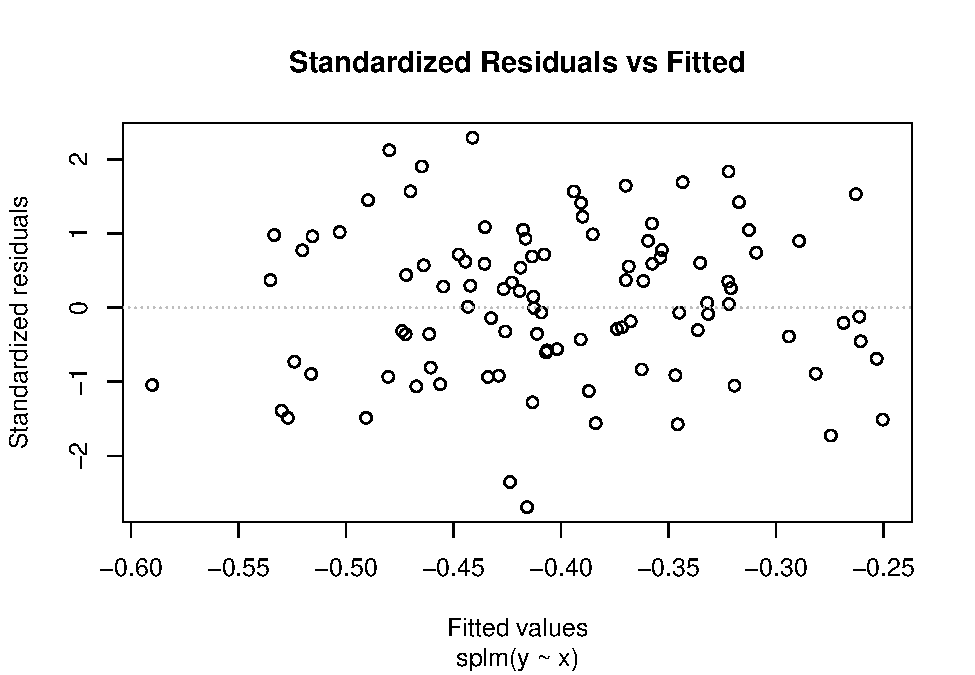
\includegraphics[width=0.49\linewidth]{preprint_files/figure-latex/unnamed-chunk-2-1}
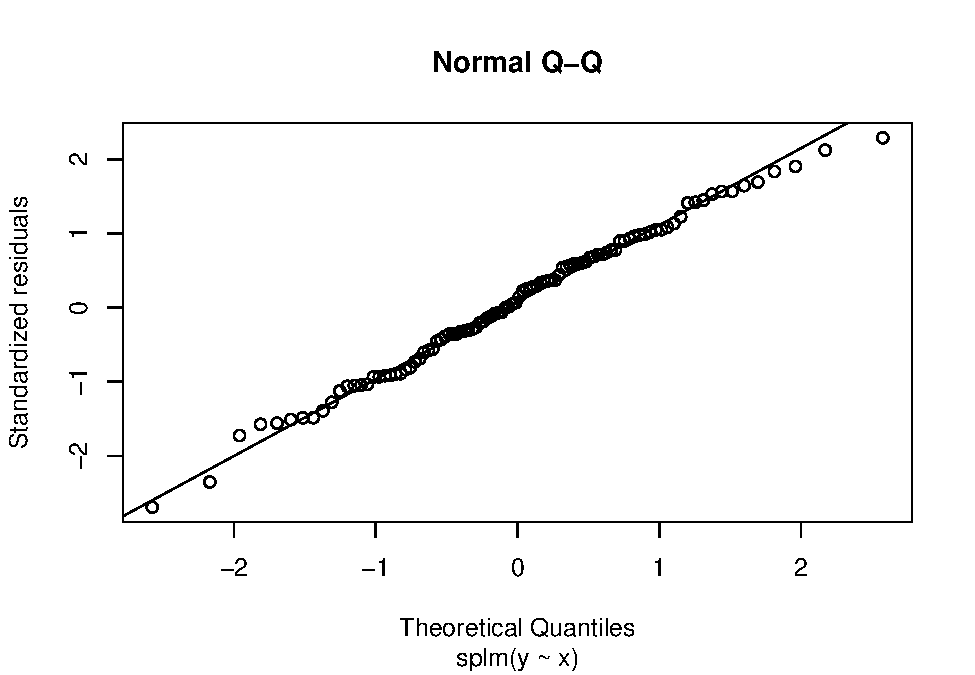
\includegraphics[width=0.49\linewidth]{preprint_files/figure-latex/unnamed-chunk-2-2}

\hypertarget{anisotropy}{%
\subsubsection{Anisotropy}\label{anisotropy}}

\begin{verbatim}
R> spmod <- splm(y ~ x, exdata, "exponential", xcoord, ycoord, anisotropy = TRUE)
\end{verbatim}

\hypertarget{prediction}{%
\subsection{Prediction}\label{prediction}}

\begin{verbatim}
R> spmod_preds <- predict(spmod, newexdata, interval = "prediction")
\end{verbatim}

\hypertarget{model-fit-statistics}{%
\subsection{Model-fit Statistics}\label{model-fit-statistics}}

\hypertarget{broom-functions}{%
\subsection{broom functions}\label{broom-functions}}

\begin{verbatim}
R> tidy(spmod)
\end{verbatim}

\begin{verbatim}
# A tibble: 2 x 5
  term        estimate std.error statistic p.value
  <chr>          <dbl>     <dbl>     <dbl>   <dbl>
1 (Intercept)  -0.391     0.364     -1.07    0.283
2 x            -0.0713    0.0738    -0.966   0.334
\end{verbatim}

\begin{verbatim}
R> glance(spmod)
\end{verbatim}

\begin{verbatim}
# A tibble: 1 x 9
      n     p  npar value   AIC  AICc logLik deviance pseudo.r.squared
  <int> <dbl> <dbl> <dbl> <dbl> <dbl>  <dbl>    <dbl>            <dbl>
1   100     2     5  244.  256.  257.  -122.       98          0.00943
\end{verbatim}

\begin{verbatim}
R> augment(spmod)
\end{verbatim}

\begin{verbatim}
# A tibble: 100 x 11
        x      y  xcoord  ycoord group subgroup .fitted  .resid   .hat .cooksd .std.resid
    <dbl>  <dbl>   <dbl>   <dbl> <fct> <fct>      <dbl>   <dbl>  <dbl>   <dbl>      <dbl>
 1 -1.12   0.602 -0.783   0.0723 1     1         -0.310  0.913  0.135  0.0642       1.05 
 2 -0.339  1.40  -0.847  -0.805  1     2         -0.366  1.77   0.0683 0.0882       1.67 
 3  2.67  -0.976 -0.0836  0.382  1     1         -0.581 -0.395  0.115  0.0500      -0.991
 4  0.842 -0.981 -0.313   0.0923 1     2         -0.451 -0.531  0.0150 0.00740     -1.00 
 5 -0.283 -0.724  0.521   0.477  1     1         -0.370 -0.353  0.0483 0.00183     -0.282
 6  0.438 -0.182  1.45   -0.703  1     2         -0.422  0.239  0.0644 0.00245      0.285
 7  0.650  0.109  0.433  -1.18   1     1         -0.437  0.546  0.0287 0.00158      0.337
 8 -0.315 -0.342 -0.0726 -2.59   1     2         -0.368  0.0262 0.0641 0.00238     -0.282
 9  0.289 -2.59   1.52   -1.11   1     1         -0.411 -2.17   0.0217 0.0771      -2.70 
10  0.315  0.383  1.21    1.05   1     2         -0.413  0.796  0.0452 0.0236       1.05 
# ... with 90 more rows
\end{verbatim}

\begin{verbatim}
R> augment(spmod, newdata = newexdata)
\end{verbatim}

\begin{verbatim}
# A tibble: 10 x 6
        x xcoord ycoord group subgroup .fitted
    <dbl>  <dbl>  <dbl> <fct> <fct>      <dbl>
 1  0.701 -0.857 -1.03  4     2         0.646 
 2 -1.45  -0.396  1.92  1     2        -0.954 
 3 -1.29  -2.05  -0.238 3     1        -0.233 
 4 -0.361  0.350 -0.243 2     2        -0.322 
 5 -0.802 -1.76  -1.98  1     2        -0.442 
 6  1.45  -1.04  -2.19  2     1        -0.504 
 7  0.218 -0.125  2.22  2     2        -0.972 
 8  0.480 -1.08   0.426 1     1        -0.0898
 9  0.908  0.378 -2.29  4     1        -0.592 
10 -0.883  1.57  -0.601 2     1        -0.173 
\end{verbatim}

\hypertarget{spatial-autoregressive-models}{%
\subsection{Spatial Autoregressive
Models}\label{spatial-autoregressive-models}}

\begin{verbatim}
R> spmod <- spautor(y ~ x, exdata_poly, "car")
\end{verbatim}

\hypertarget{neighborhood-indexing-for-big-data}{%
\subsection{Neighborhood Indexing for Big
Data}\label{neighborhood-indexing-for-big-data}}

\begin{verbatim}
R> spmod <- splm(y ~ x, exdata, "exponential", xcoord, ycoord, local = TRUE)
\end{verbatim}

\hypertarget{the-local-list}{%
\subsubsection{The local list}\label{the-local-list}}

\begin{verbatim}
R> spmod <- splm(y ~ x, exdata, "exponential", xcoord, ycoord, local = list(parallel = TRUE))
\end{verbatim}

\hypertarget{random-effects}{%
\subsection{Random Effects}\label{random-effects}}

\begin{verbatim}
R> spmod <- splm(y ~ x, exdata, "exponential", xcoord, ycoord, random = ~ group)
\end{verbatim}

\hypertarget{partition-factors}{%
\subsection{Partition Factors}\label{partition-factors}}

\begin{verbatim}
R> spmod <- splm(y ~ x, exdata, "exponential", xcoord, ycoord, partition_factor = ~ group)
\end{verbatim}

\hypertarget{initial-values-and-known-values}{%
\subsection{Initial Values and Known
Values}\label{initial-values-and-known-values}}

\begin{verbatim}
R> spcov_params_init <- spcov_initial("exponential", de = 1, ie = 0, known = "ie")
R> spmod <- splm(
+   y ~ x,
+   exdata,
+   spcov_initial = spcov_params_init,
+   xcoord = xcoord, 
+   ycoord = ycoord
+ )
\end{verbatim}

\hypertarget{simulating-gaussian-random-variables}{%
\subsection{Simulating Gaussian Random
Variables}\label{simulating-gaussian-random-variables}}

\begin{verbatim}
R> spcov_params_val <- spcov_params("exponential", de = 1, ie = 1, range = 2)
R> var <- sprnorm(spcov_params_val, data = exdata, xcoord = xcoord, ycoord = ycoord)
\end{verbatim}

\hypertarget{discussion}{%
\section{Discussion}\label{discussion}}

\hypertarget{data-and-code-availability}{%
\section*{Data and Code Availability}\label{data-and-code-availability}}
\addcontentsline{toc}{section}{Data and Code Availability}

\hypertarget{acknowledgements}{%
\section*{Acknowledgements}\label{acknowledgements}}
\addcontentsline{toc}{section}{Acknowledgements}

\hypertarget{references}{%
\section*{References}\label{references}}
\addcontentsline{toc}{section}{References}

\hypertarget{refs}{}
\leavevmode\hypertarget{ref-cressie1985fitting}{}%
Cressie, Noel. 1985. ``Fitting Variogram Models by Weighted Least
Squares.'' \emph{Journal of the International Association for
Mathematical Geology} 17 (5): 563--86.

\leavevmode\hypertarget{ref-cressie1993statistics}{}%
---------. 1993. \emph{Statistics for Spatial Data}. John Wiley \& Sons.

\leavevmode\hypertarget{ref-curriero1999composite}{}%
Curriero, Frank C, and Subhash Lele. 1999. ``A Composite Likelihood
Approach to Semivariogram Estimation.'' \emph{Journal of Agricultural,
Biological, and Environmental Statistics}, 9--28.

\leavevmode\hypertarget{ref-harville1977maximum}{}%
Harville, David A. 1977. ``Maximum Likelihood Approaches to Variance
Component Estimation and to Related Problems.'' \emph{Journal of the
American Statistical Association} 72 (358): 320--38.

\leavevmode\hypertarget{ref-patterson1971recovery}{}%
Patterson, H Desmond, and Robin Thompson. 1971. ``Recovery of
Inter-Block Information When Block Sizes Are Unequal.''
\emph{Biometrika} 58 (3): 545--54.

\leavevmode\hypertarget{ref-wolfinger1994computing}{}%
Wolfinger, Russ, Randy Tobias, and John Sall. 1994. ``Computing Gaussian
Likelihoods and Their Derivatives for General Linear Mixed Models.''
\emph{SIAM Journal on Scientific Computing} 15 (6): 1294--1310.

\bibliographystyle{unsrt}
\bibliography{references.bib}


\end{document}
